\section{Hadoop 2.2}
\label{sec:hadoop-2.2}

\par A partir des versions , Hadoop vient avec un nouveau composant appelé Yarn. 

\begin{figure}[h!]
  \centering
  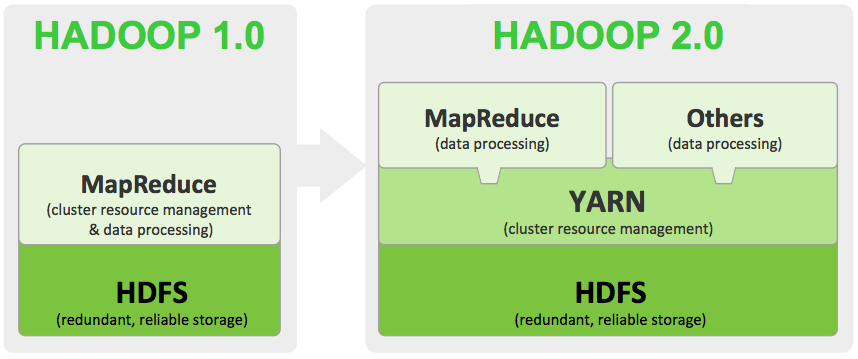
\includegraphics[width=12cm]{images/yarn.png}
  \caption{Différences entre Hadoop 1.x et Hadoop 2.x}
  \label{fig:yarn}
\end{figure}

Yarn est responsable de la gestion des ressources, et utilise des processus similaires pour leur gestion. Le NodeManager vient remplacer le TaskTracker, qui s'occupe de faire le lien entre le DataNode et le ResourceManager localisé sur le master (NameNode). Le ResourceManager déploie les applications sur les noeuds grâce à sa communication avec les NodeManagers.

--> Schéma Hadoop Yarn

\subsection{Connexion sur un ordinateur à Supélec}
\label{sec:connexion-sur-un}

\par La connexion avec un compte utilisateur précis est particulière, dans la mesure où on peut accéder à son dossier personnel, correspondant à des identifiants de connexion, depuis n'importe quelle machine. En effet, une machine est responsable de la gestion des logins, et contient les données personnelles correspondantes. Ces données transitent lors d'une connexion, ce qui peut faire croire que ces données sont présentes sur tous les ordinateurs.

\par Il est important de garder à l'esprit ce mécanisme, car c'est grâce à celui-ci que nous pourront simplifier la configuration de Hadoop sur le cluster Skynet. Malgré ces données qui ne sont pas propres à une machine, nous devons également pouvoir accéder à la mémoire de la machine physique, afin de pouvoir les utiliser comme DataNodes. Dans un premier temps, nous utiliserons le dossier \texttt{/tmp} accessible en lecture écriture à n'importe qui (donc peu sécurisé, mais adapté à notre installation de test).

\begin{figure}[h!]
  \centering
  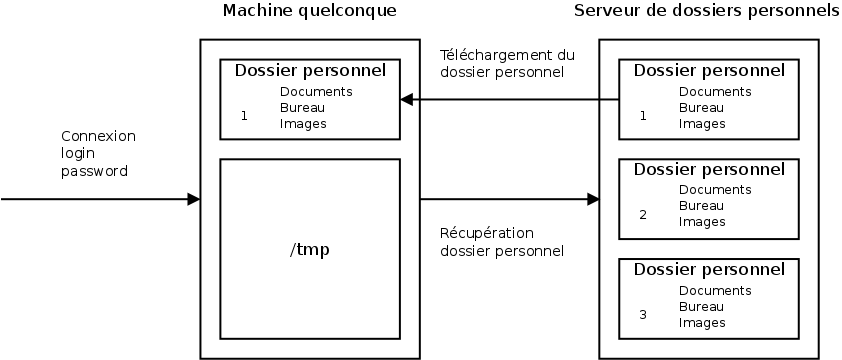
\includegraphics[width=16cm]{images/connexion_supelec.png}
  \caption{Exemple d'une connexion sur une machine quelconque}
  \label{fig:connexion_supelec}
\end{figure}

\subsection{Connexion SSH}
\label{sec:connexion-ssh}

\par Lors d'une connexion SSH, le fichier \texttt{.bash\_profile} est executé. Lors d'un login, c'est le fichier \texttt{.bashrc} qui est exécuté. Comme toutes les connexions via hadoop se font par ssh, nous allons les lier tous les deux. Pour cela, on créera un fichier \texttt{.bash\_profile} contenant au moins :

\begin{minted}[frame=single,linenos,mathescape]{bash}
  if [ -f .bashrc ]; then
    . ~/.bashrc
  fi
\end{minted}

\par De cette manière, si le fichier \texttt{.bashrc} existe, on le charge, sinon on ne fait rien.
\par On se connecte successivement sur \texttt{Ghome}, puis \texttt{Term2} :
\begin{minted}[frame=single,linenos,mathescape]{bash}
  Alex > ssh ghome
  Last login: Sat Jun 14 22:00:38 2014 from 193.48.225.99
  Alex [gserver] > ssh term2
  Last login: Sat Jun 14 20:52:34 2014 from gserver.grid.metz.supelec.fr
  Alex [term2] > 
\end{minted}

\par A partir de \texttt{Term2}, on peut se connecter à chacune des machines du cluster Skynet, dont les alias permettent de simplifier les opérations. Ainsi au lieu de 

\begin{minted}{bash}
  ssh careil_ale@term2.grid.metz.supelec.fr
\end{minted}
 on peut simplement faire
\begin{minted}{bash}
  ssh careil_ale@term2
\end{minted}

car nous sommes dans le domaine \texttt{grid.metz.supelec.fr}.

 Il est inutile de spécifier le nom d'utilisateur lors de la connexion puisque, comme expliqué précédemment, notre compte existe sur toutes les machines (pas physiquement, mais il est chargé à chaque fois). Donc au lieu de se connecter avec la commande précédente, on peut simplement faire :
 
\begin{minted}{bash}
  ssh term2
\end{minted}

Cependant, il faut effectuer une manoeuvre afin de pouvoir se connecter facilement sans mot de passe. En effet, on va générer une clé SSH avec la commande \texttt{ssh-keygen} (qu'on appellera \texttt{id\_rsa\_test}). Vu qu'on ne veut pas utiliser de mot de passe pour se connecter, on omettra la \texttt{Passphrase} lors de la création de la clé.

\begin{verbatim}
Alex > ssh-keygen
Generating public/private rsa key pair.
Enter file in which to save the key (/home/alexandre/.ssh/id_rsa): id_rsa_test
Enter passphrase (empty for no passphrase): 
Enter same passphrase again: 
Your identification has been saved in id_rsa_test.
Your public key has been saved in id_rsa_test.pub.
The key fingerprint is:
61:e0:38:43:34:aa:fc:7b:6e:e3:04:79:a2:f6:14:1a alexandre@gentooalex
The key's randomart image is:
+--[ RSA 2048]----+
|   .+ .          |
|   o + .         |
|  . + . o        |
|..  .o . .       |
|.E = .  S        |
|  = =            |
| + o .           |
|. o o+           |
|   o=o.          |
+-----------------+
\end{verbatim}

\par Maintenant, allons dans le dossier \texttt{.ssh} contenant notre clé publique, et notre clé privée afin de créer le fichier \texttt{authorized\_keys} s'il n'existe pas déjà. S'il n'existe pas, tapez la commande \texttt{touch authorized\_keys} afin de le créer.

\par On va ajouter notre clé publique à l'ensemble des clés autorisées :
\begin{verbatim}
cat id_rsa_test.pub >> authorized_keys
\end{verbatim}
\par On peut désormais vérifier que cela fonctionne bien en se connectant par exemple à \texttt{sh00}. Normalement, aucun mot de passe n'est demandé. 

\par Un dernier problème peut empêcher une connexion directe en ssh, celui de la vérification d'authenticité de l'hôte sur lequel on veut se connecter : 
\begin{verbatim}
Juan [master] > ssh munozperez_jua@ghomE.metz.supelec.fr
The authenticity of host 'ghome.metz.supelec.fr (193.48.224.129)' 
can't be established.
RSA key fingerprint is c1:41:c3:6d:f1:21:a2:2a:e6:30:b0:60:f7:de:22:b1.
Are you sure you want to continue connecting (yes/no)? YES
Warning: Permanently added 'ghome.metz.supelec.fr,193.48.224.129' 
(RSA) to the list of known hosts.
Last login: Sun Apr  6 21:20:11 2014 from 193.48.225.99
\end{verbatim}

\par Pour enlever ce message, il faut se connecter manuellement à chaque noeud pour qu'il soit ajouté à la liste des hôtes connus (listés dans le fichier \texttt{~/.ssh/known_hosts}).


%%% Local Variables: 
%%% mode: latex
%%% TeX-master: "CompteRendu"
%%% End: 
